\documentclass[uplatex,a4j,11pt,dvipdfmx]{jsarticle}
\usepackage{listings,jvlisting}
\bibliographystyle{junsrt}

\usepackage{url}

\usepackage{graphicx}
\usepackage{gnuplot-lua-tikz}
\usepackage{pgfplots}
\usepackage{tikz}
\usepackage{amsmath,amsfonts,amssymb}
\usepackage{bm}
\usepackage{siunitx}

\makeatletter
\def\fgcaption{\def\@captype{figure}\caption}
\makeatother
\newcommand{\setsections}[3]{
\setcounter{section}{#1}
\setcounter{subsection}{#2}
\setcounter{subsubsection}{#3}
}
\newcommand{\mfig}[3][width=15cm]{
\begin{center}
\includegraphics[#1]{#2}
\fgcaption{#3 \label{fig:#2}}
\end{center}
}
\newcommand{\gnu}[2]{
\begin{figure}[hptb]
\begin{center}
\input{#2}
\caption{#1}
\label{fig:#2}
\end{center}
\end{figure}
}
\newcommand{\gaa}{\gamma_{AA}}
\newcommand{\gbb}{\gamma_{BB}}
\newcommand{\gab}{\gamma_{AB}}

\begin{document}
\title{磁性物理学 レポート No.3}
\author{82311971 佐々木良輔}
\date{}
\maketitle
\subsection*{(1)}
図のように副格子Aの向く方向を正として,外部磁場は正の方向にかけるものとする.
外部磁場$H_{\rm ext}$が無い状態での副格子$A$, $B$磁化を$M_0$とする.
磁場を印加した際の副格子$A$, $B$それぞれについて,磁化の変化量を$\delta M_A$, $\delta M_B$とすると,
磁場中での副格子$A$, $B$の磁化は
\begin{align}
  \begin{split}
    M_A=M_0+\delta M_A\\
    M_B=-M_0+\delta M_B
  \end{split}
\end{align}
である.このとき副格子$A$が$B$から受ける分子場は
\begin{align}
  H_w^A=-\gamma M_B=-\gamma(-M_0+\delta M_B)
\end{align}
また$B$が$A$から受ける分子場は
\begin{align}
  H_w^B=-\gamma M_A=-\gamma(M_0+\delta M_A)
\end{align}
である.ここで図2のように外部磁場が無い状態での平衡位置を$\alpha_0$, $-\alpha_0$とする.
ただし外部磁場0のときの磁化が$M_0$なので$\alpha_0=\beta m\gamma M_0$である.
外部磁場を印加したときの平衡状態からのズレを$\delta\alpha_A$, $\delta\alpha_B$とすると
\begin{align}
  \begin{split}
    \delta\alpha_A&=\beta m(H_{\rm ext}+H_w^A)-\alpha_0\\
    &=\beta m(H_{\rm ext}-\gamma\delta M_B)+\beta m\gamma M_0-\alpha_0\\
    &=\beta m(H_{\rm ext}-\gamma\delta M_B)
  \end{split}
\end{align}
同様にして
\begin{align}
  \begin{split}
    \delta\alpha_B&=\beta m(H_{\rm ext}+H_w^B)-(-\alpha_0)\\
    &=\beta m(H_{\rm ext}-\gamma\delta M_A)
  \end{split}
\end{align}
である.ここで$\delta\alpha\ll1$のとき,
$M$を$\alpha_0$周りで1次までテイラー展開することで
\begin{align}
  M(\alpha_0+\delta\alpha)=NmL(\alpha_0)+NmL'(\alpha_0)\delta\alpha
\end{align}
これを用いて$\delta M_A$, $\delta M_B$は
\begin{align}
  \begin{split}
    \delta M_A&=M(\alpha_0+\delta\alpha_A)-M(\alpha_0)\\
    &=NmL'(\alpha_0)\beta m(H_{\rm ext}-\gamma\delta M_B)\\
    &=\frac{Nm^2}{k_BT}L'(\alpha_0)(H_{\rm ext}-\gamma\delta M_B)
  \end{split}
\end{align}
\begin{align}
  \begin{split}
    \delta M_B&=\frac{Nm^2}{k_BT}L'(\alpha_0)(H_{\rm ext}-\gamma\delta M_A)
  \end{split}
\end{align}
正味の磁化は$M=\delta M_A+\delta M_B$なので(7), (8)の両辺を足すと
\begin{align}
  \begin{array}{cc}
    &M=\cfrac{Nm^2}{k_BT}L'(\alpha_0)(2H_{\rm ext}-\gamma M)\\
    \iff&M\left(1+\cfrac{\gamma Nm^2L'(\alpha_0)}{k_BT}\right)=\cfrac{2Nm^2}{k_BT}L'(\alpha_0)H_{\rm ext}
  \end{array}
\end{align}
したがって磁気感受率は
\begin{align}
  \begin{split}
    \chi=\frac{M}{H_{\rm ext}}&=\frac{\frac{2Nm^2}{k_BT}L'(\alpha_0)}{1+\frac{\gamma Nm^2L'(\alpha_0)}{k_BT}}\\
    &=\frac{2Nm^2L'(\alpha_0)}{k_BT+\gamma Nm^2L'(\alpha_0)}
  \end{split}
\end{align}
となる.ここで$\alpha_0=0$では$L'(0)=1/3$なので
\begin{align}
  \begin{split}
    \chi&=\frac{\frac{2Nm^2}{3k_B}}{T+\frac{\gamma Nm^2}{3k_B}}=:\frac{C}{T+T_N}
  \end{split}
\end{align}
ここで$C=2Nm^2/3k_B$, $T_N=\gamma Nm^2/3k_B$とした.
$T=T_N$のときは
\begin{align}
  \chi=\frac{1}{\gamma}
\end{align}
となる.
\begin{center}
  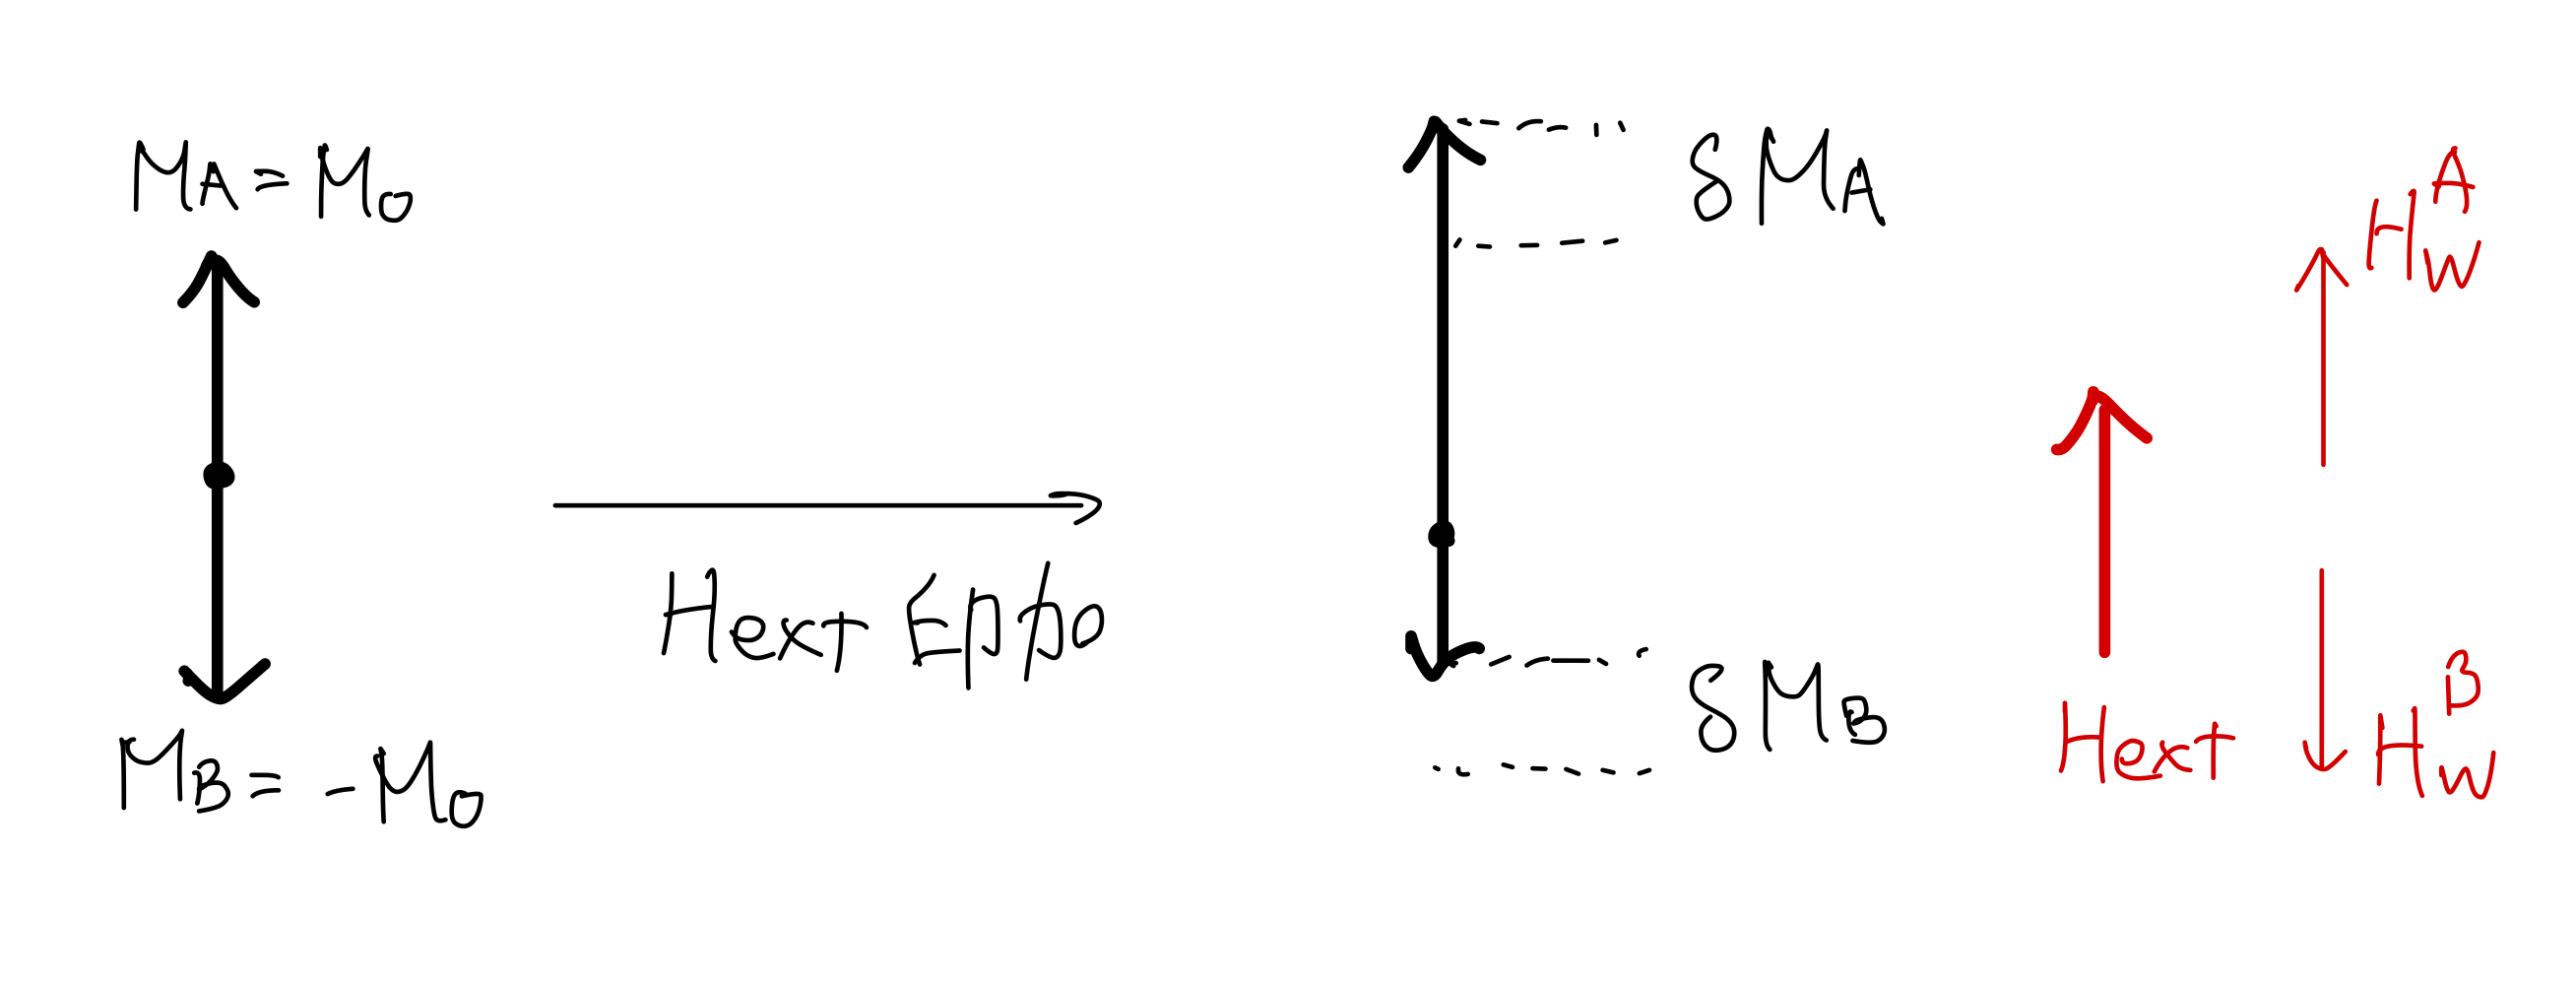
\includegraphics[width=8cm]{1_coord.png}
  \fgcaption{反強磁性体に磁場を印加した際の磁化の挙動}
\end{center}
\begin{center}
  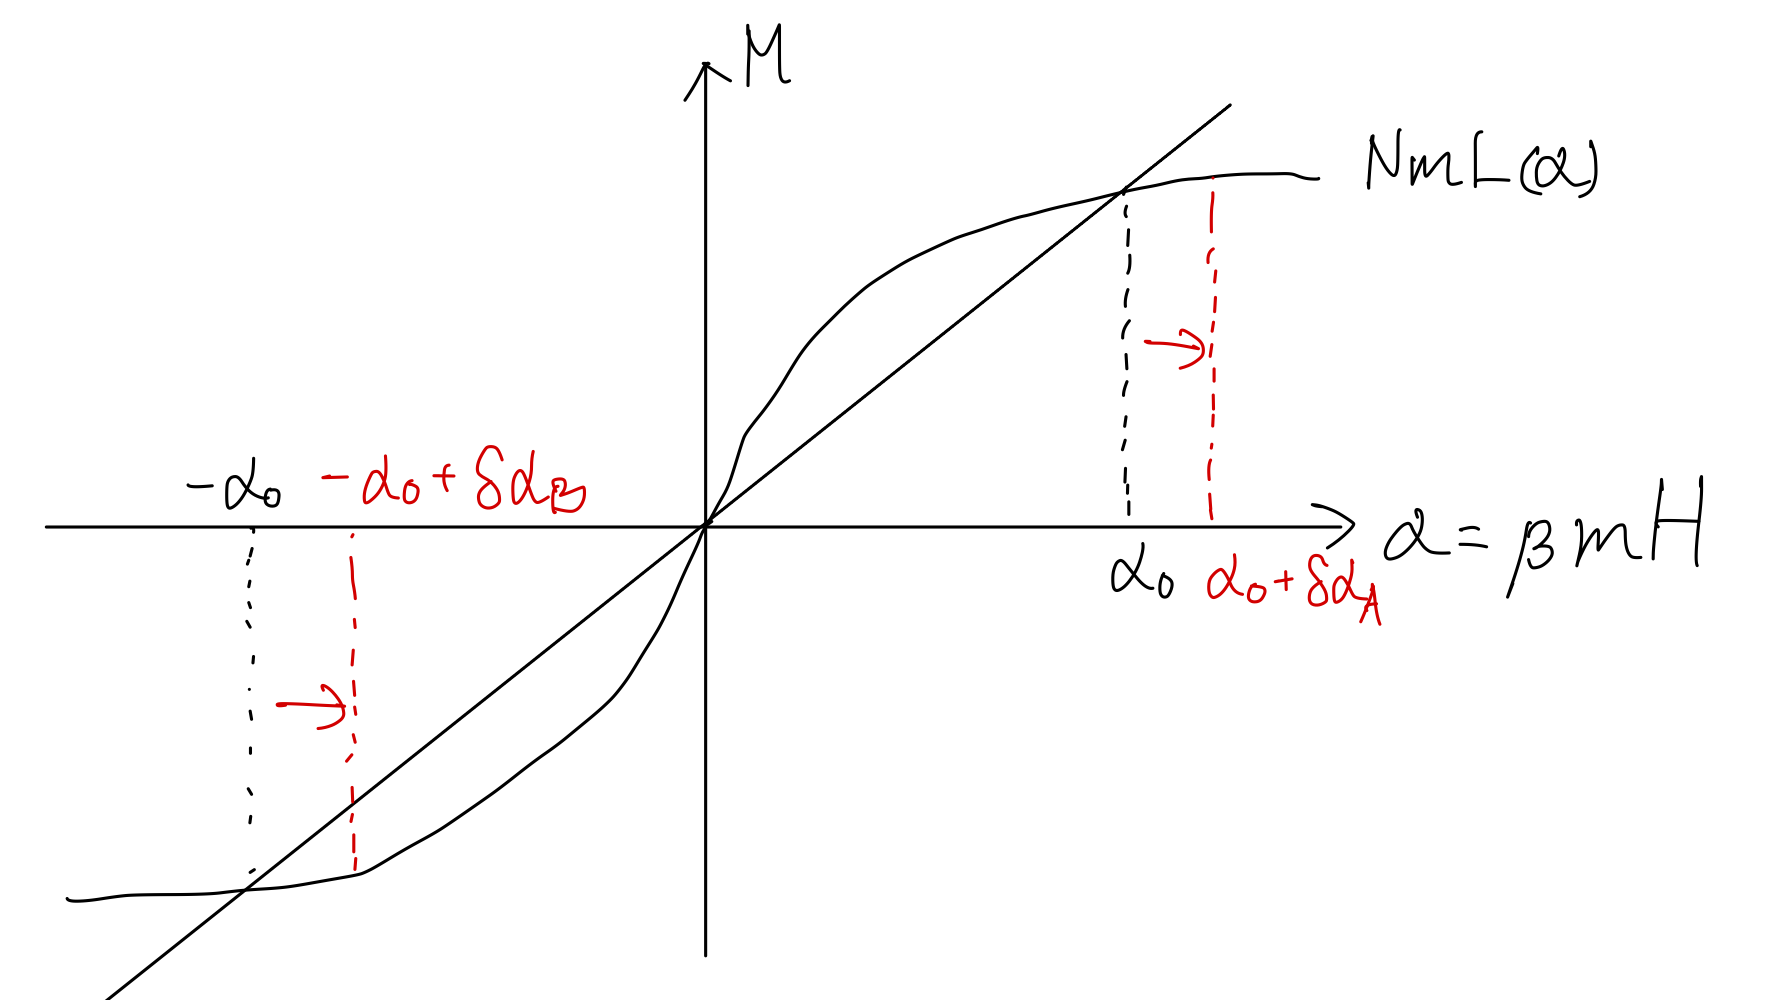
\includegraphics[width=12cm]{1_HM.png}
  \fgcaption{外部磁場による自己無撞着解の変化}
\end{center}
\subsection*{(2)}
副格子$A$, $B$の磁化はそれぞれ
\begin{align}
  \begin{split}
    M_A&=\frac{C}{T}(H_{\rm ext}+H_w^A)\\
    &=\frac{C}{T}\left(H_{\rm ext}+{\gaa}M_A-{\gab}M_B\right)
  \end{split}
\end{align}
\begin{align}
  \begin{split}
    M_B&=\frac{C}{T}(H_{\rm ext}+H_w^B)\\
    &=\frac{C}{T}\left(H_{\rm ext}+{\gbb}M_B-{\gab}M_A\right)
  \end{split}
\end{align}
であった.ここで簡単のため$M_A=x$, $M_B=y$, $C{\gaa}/T=a$,
$C{\gbb}/T=b$, $C{\gab}/T=c$, $CH_{\rm ext}/T=h$と置くと
\begin{align}
    &\left\{
    \begin{array}{c}
      x=h+ax-cy\\
      y=h+by-cx
    \end{array}\right.\\
    \iff&\left\{
    \begin{array}{c}
      x=\cfrac{h-cy}{1-a}\\
      y=\cfrac{h-cx}{1-b}
    \end{array}\right.
\end{align}
(16)から
\begin{align}
  \begin{array}{cc}
    &y=\cfrac{h}{1-b}-\cfrac{c}{1-b}\cfrac{h-cy}{1-a}=\cfrac{h(1-a-c)+c^2y}{(1-a)(1-b)}\\
    \iff&y\left(1-\cfrac{c^2}{(1-a)(1-b)}\right)=\cfrac{h(1-a-c)}{(1-a)(1-b)}\\
    \iff&y=\cfrac{h(1-a-c)}{1-a-b+ab-c^2}
  \end{array}
\end{align}
$x$については$a$と$b$を入れ替えれば
\begin{align}
  x=\frac{h(1-b-c)}{1-a-b+ab-c^2}
\end{align}
である.正味の磁化は$M=M_A+M_B=x+y$なので
\begin{align}
  \begin{array}{cc}
    &x+y=\frac{h(2-a-b-2c)}{1-a-b+ab-c^2}\\
    \iff&\cfrac{h}{x+y}=\cfrac{1-a-b+ab-c^2}{2-a-b-2c}\\
    \iff&\cfrac{\frac{C}{T}H_{\rm ext}}{M}=\cfrac{1-\frac{C}{T}{\gaa}-\frac{C}{T}{\gbb}+\left(\frac{C}{T}\right)^2{\gaa}{\gbb}-\left(\frac{C}{T}\right)^2{\gab}^2}{2-\frac{C}{T}{\gaa}-\frac{C}{T}{\gbb}-2\frac{C}{T}{\gab}}\\
    \iff&\cfrac{H_{\rm ext}}{M}=\cfrac{\frac{T}{C}-({\gaa}+{\gbb})+\frac{C}{T}\left({\gaa}{\gbb}-{\gab}^2\right)}{2-\frac{C}{T}({\gaa}-{\gbb}-2{\gab})}
  \end{array}
\end{align}
を得る.
また$1/\chi_D=(2{\gab}-{\gaa}-{\gbb})/4$, $b=C({\gaa}-{\gbb})^2/8$, $\theta=C({\gaa}+{\gbb}+2{\gab})/2$とおいたとき
\begin{align}
  \begin{split}
    \frac{T}{2C}+\frac{1}{\chi_D}-\frac{b}{T-\theta}&=\frac{T}{2C}+\frac{2{\gab}-{\gaa}-{\gbb}}{4}-\frac{\frac{C}{4T}({\gaa}-{\gbb})^2}{2-\frac{C}{T}({\gaa}+{\gbb}+2{\gab})}\\
    &=\frac{1}{2-\frac{C}{T}(\gaa+{\gbb}+2{\gab})}\biggl(-\frac{C(\gaa-\gbb)^2}{4T}\\
      &\qquad+\frac{2\gab-\gaa-\gbb}{4}\left(2-\frac{C}{T}(\gaa+\gbb+2\gab)\right)\\
      &\qquad+\frac{T}{2C}\left(2-\frac{C}{T}(\gaa+\gbb+2\gab)\right)\biggr)\\
    &=\frac{1}{2-\frac{C}{T}(\gaa+{\gbb}+2{\gab})}
      \biggl(-\frac{C}{4T}\gaa^2+\frac{C}{2T}\gaa\gbb-\frac{C}{4T}\gbb^2\\
      &\qquad+\gab-\frac{\gaa}{2}-\frac{\gbb}{2}-\frac{C}{4T}\left(4\gab^2-(\gaa+\gbb)^2\right)\\
      &\qquad+\frac{T}{C}-\frac{1}{2}\left(\gaa+\gbb+2\gab\right)\biggr)\\
    &=\frac{1}{2-\frac{C}{T}(\gaa+{\gbb}+2{\gab})}
      \biggl(-\frac{C}{4T}\gaa^2+\frac{C}{2T}\gaa\gbb-\frac{C}{4T}\gbb^2\\
      &\qquad+\gab-\frac{\gaa}{2}-\frac{\gbb}{2}-\frac{C}{T}\gab^2+\frac{C}{4T}\left(\gaa^2+2\gaa\gbb+\gbb^2\right)\\
      &\qquad+\frac{T}{C}-\frac{1}{2}\left(\gaa+\gbb+2\gab\right)\biggr)\\
    &=\frac{1}{2-\frac{C}{T}(\gaa+{\gbb}+2{\gab})}
      \biggl(0+\frac{C}{T}\gaa\gbb-0\\
      &\qquad+0-\gaa-\gbb-\frac{C}{T}\gab^2+\frac{T}{C}\biggr)\\
    &=\frac{\frac{T}{C}-({\gaa}+{\gbb})+\frac{C}{T}\left({\gaa}{\gbb}-{\gab}^2\right)}{2-\frac{C}{T}({\gaa}-{\gbb}-2{\gab})}
  \end{split}
\end{align}
以上から
\begin{align}
  \frac{H_{\rm ext}}{M}=\frac{T}{2C}+\frac{1}{\chi_D}-\frac{b}{T-\theta}
\end{align}
である.
\end{document}